\chapter{Intrusion Detection}
\begin{figure}[htbp]
   \centering
   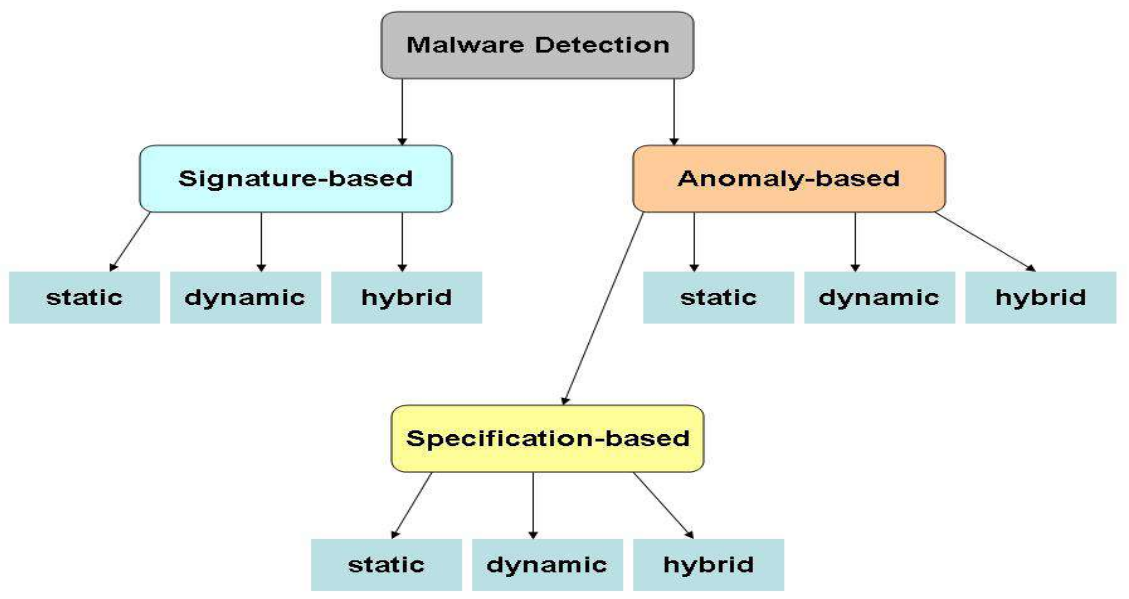
\includegraphics{images/IntrusionDetection_schema.png}
   \caption{Intrusion Detection Taxonomy}
   \label{fig:IntrusionDetection_taxonomy}
\end{figure}

\labelitemize{
   \textbf{INPUT-EVENTS}
}{
   \begin{enumerate}
      \item End-point events
         \begin{enumerate}
            \item  Invocation to OS
            \item  Memory analysis
            \item  Files that are downloaded
            \item  Programs that are executed
         \end{enumerate}
      \item Network events
         \begin{enumerate}
            \item Contents of packets that are transmitted
            \item Information transmitted on a circuit
         \end{enumerate}
      \end{enumerate}
      }
      
\textbf{Networks events} are generated by a module that monitors ongoing communication, i.e. a \textbf{packer sniffer}.\\
This poses two problems:
\begin{enumerate}
   \item \textit{Lost messages}, since the sniffer cannot slow down the communication it is sniffing
   \item \textit{Assumptions} on the \textit{behavior} of the receiving node
\end{enumerate}
There are \textit{\textbf{evasion} attacks} where the attacker transmits \textbf{fake packets} to increase the computational load od the detection,
exploiting fake checksum, overlapping fragments etc.

\section{Anomaly Based}
The behavior of the target system is observed for a time interval and a \textbf{learning model} is built representing the \textit{normal} behavior.\\
Note that \textbf{learning} implies discovering parameters such as:
\begin{itemize}
   \item \textbf{Services} that are used and time of the usage
   \item When users \textbf{log in} and the length of their \textbf{sessions}
   \item User \textbf{requests} and \textbf{OS functions} they invoke
   \item Computation and communication \textbf{bandwidths} used
\end{itemize}
After the learning phase, any behavior that is too \textit{far} from the model that has
been built is defined as an \textbf{anomaly} due to an \textit{ongoing intrusion}.\nl
Clearly the critical parameters are the amount of \textbf{information} acquired during the learning phase and the \textbf{threshold} on the \textit{"distance"}.
Sometimes continuous learning is preferred since the normal behavior \textbf{changes} as time passes.

\begin{enumerate}
   \item \textbf{Dynamic}:
   Information on a program behavior are collected by executing the program
   \item \textbf{Static}:
   A static analysis returns information on the program behavior\\
   e.g. the OS functions it calls, information on the call order, etc.
   \item \textbf{Hybrid}:
   Dynamic collection of information to cover lack of information in the output of the static analysis
\end{enumerate}

\subsection{Specification Based}
The key point here is that the so-called normal network behaviour is not deduced by observing programs behaviour over time,
instead by what are the running programs and what they should do according to their specification.

\section{Signature Based}

The main idea is that there are some \textbf{behaviors} and some \textbf{data} in a \textit{malware} that \textbf{identify}
the malware in a reliable way, i.e. \textit{malware signature}.\\
All the signatures are stored in a database that is used to discover malware,
hence two issues arise:
\begin{enumerate}
   \item How to discover a signature
   \item How to update the database
\end{enumerate}
Note that this kind of detection needs malware signatures, thus it cannot detect an attack exploiting a 0-day vulnerability.

A 0-day exploit can be discovered through anomaly detection or by analyzing the
information that a {---}for-intelligence-{---} honeypot  returns,
however thare also alternative strategies exist to define a signature,
for instance
extending the approach by uploading suspicious code on the system of the tool supplier when a partial matching occurs.
This is a solution inspired by \textit{default allow},
i.e. anything that does not match the signature is allowed.\nl

Signature based detection methods can be classified as follows
\begin{enumerate}
   \item \textbf{Dynamic}:
   The program runs in a protected environment (virtual machine or sandbox), 
   and then the collected information is compared against the signature
   \item \textbf{Static}:
   The program code is analyzed, and the output is compared against the signature.\\
   This was the standard approach in old antivirus tools, which nowdays instead apply a hybrid one
   \item \textbf{Hybrid}:
   Merge of the two previous approaches:
   a static analysis collects suspicious programs and then the behavior of each program is monitored.
\end{enumerate}

A simple antivirus scanner performing \textbf{static} analysis
matches code fragments against signatures, uses heuristic strategies to discover viruses and polymorphic viruses,
and performs 
integrity checks on files to discover malicious updates by pairing files with checksum, hash, keyed hash etc.

\textbf{Dynamic} solutions typically use a \textit{decryption and emulation} approach:
The suspicious code is uploaded on a remote system 
(cloud run by the antivirus supplier)
which emulates the execution for a predefined number of
instructions.
If the executions yields the expected results,
the code is classified as safe.
Clearly this does not discover viruses hidden within normal code.